% !TeX spellcheck = ru_RU
% !TeX encoding = UTF-8
\section{Технология SigFox}
\subsection{Назначение системы}
Компания \textbf{Sigfox} (Франция) занимается разработкой и внедрением технологии сверх узкополосной (\textbf{UNB} — Ultra Narrow Band) беспроводной связи для передачи данных в субгигагерцовом нелицензируемом диапазоне 868.8 MГц. Сеть компаний развернута в Европе: Франция, Италия, Великобритания, Ирландия, Испания, Португалия, Люксембург, Нидерланды, Бельгия, Дания. 

Основная разработка Sigfox — энергоэкономные беспроводные сети, которые станут основой интернета вещей. Благодаря этим сетям между собой смогут обмениваться данными «умные» часы, телевизоры, микроволновые печи, стиральные машины и другие устройства. Эта технология изначально предназначена для связи на низких скоростях передачи данных. SigFox в настоящее время использует самый популярный европейский \textbf{ISM} диапазон на 868 МГц (как определено стандартом ETSI и СЕРТ), а также 902 МГц в США (как определено FCC), в зависимости от конкретных региональных правил. Система развернута с использованием возможностей современных сотовых сетей.
\subsection{Структура системы}
Устройство может отправить до 140 сообщений в день, и каждое сообщение может содержать до 12 байт полезных данных. 12 байт покрывает потребности устройств, которые передают данные, такие как местоположение устройства, индекс потребления энергии, сигнал тревоги или любой другой тип основной сенсорной информации. 
Также можно передавать до 4 сообщений из 8 байт полезных данных на каждое устройство в сутки. Для того, чтобы получать сообщения, устройство должно запросить данные с сервера, это должно быть запрограммировано на конкретные события или на определенное время, что позволяет экономить энергию, находясь большую часть времени в спящем режиме. 8 байт, отправленные на устройство, позволяют при необходимости отправить данные конфигурации, можно оптимизировать срок службы аккумулятора. Этого достаточно, если нет необходимости в полноценной двусторонней связи. На данный момент система Sigfox реализована с односторонней связью: данные с датчиков агрегируются и передаются на сервера компании Sigfox(\ref{fig:img11}). 
\begin{figure}[H]
	\centering
	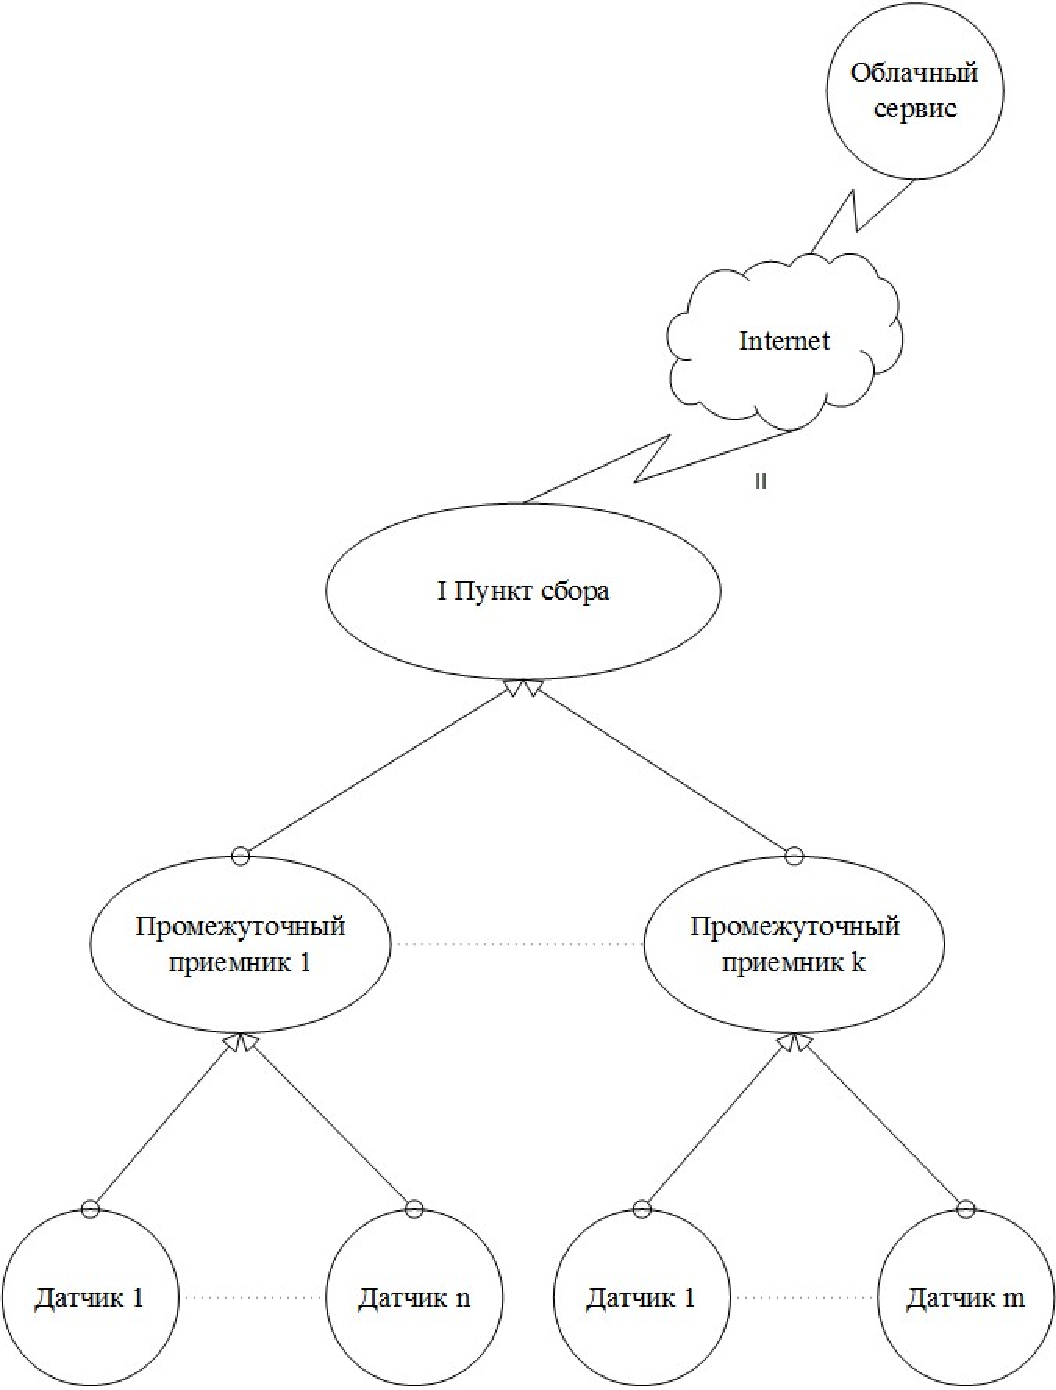
\includegraphics[width=0.5\textwidth]{img/kich_bur/11.pdf}
	\caption{Стурктура системы Sigfox}
	\label{fig:img11}
\end{figure}
\subsection{Разбиение системы на уровни}
Sigfox — исторически первая крупная компания на рынке интернета вещей — выбрала для себя довольно закрытую модель. На рисунке \ref{fig:img12} представлено разбиение системы на уровни. У Sigfox необходимо купить базовые станции и заключить с ним договор на разворачивание сети, к которой будет предоставляться платный доступ сторонним абонентам. Базовые станции передают данные на сервера Sigfox, то есть канал связи --- не физический, но логический и ПО верхнего уровня также принадлежат Sigfox. Sigfox не стал узурпировать рынок чипов и конечных устройств --- он договорился с Texas Instruments, SiLabs и другими производителями о поддержке своей сети, что позволяет заказать какое-то нестандартное Sigfox-устройство. К сожалению, проблему может составить его подключение к сети: если в Европе Sigfox успел развернуться, то сейчас, с появлением LoRa, его экспансия фактически остановилась.
Сотовые сети LPWAN --- сети масштаба городов --- это сети с множеством базовых
станций (например, на покрытие Москвы надо порядка 200 штук), как правило, обслуживаемые оператором сети, предоставляющим за деньги доступ к ней владельцам конечных устройств. Sigfox устанавливает жесткую тарифную сетку. 
\begin{figure}[H]
	\centering
	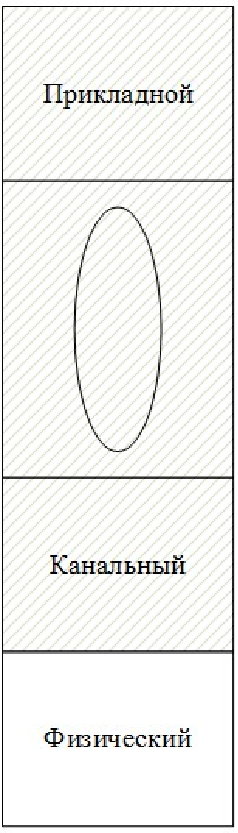
\includegraphics[width=0.2\textwidth]{img/kich_bur/12.pdf}
	\caption{Разбиение системы Sigfox на уровни}
	\label{fig:img12}
\end{figure}
Таким образом, все уровни закрыты, за исключением физического, что позволяет
сделать гибкую сетку маломощных устройств. 
\subsection{Особенности построения уровней}
Sigfox не поддерживает топологию «звезда». Ни в Sigfox, ни в «Стриже», ни вообще в мире узкополосных UNB-систем сети такой топологии технически невозможны: из-за специфики UNB-систем абонентское устройство в общем случае не может принимать данные в произвольные моменты времени от других абонентских устройств, а значит, не может выступать в качестве ретранслятора.
Все решения распадаются на две группы: широкополосные UWB (Ultra Wide Band, к ним из перечисленного относится только LoRa) и узкополосные UNB (Ultra Narrow Band, в нашем случае это Sigfox и «Стриж»). Из этого проистекает ряд отличий.
UWB: один канал занимает полосу в эфире с шириной 125 или 250 кГц
UNB: один канал занимает полосу в эфире с шириной 100 Гц

В России в диапазоне, условно именуемом «\textbf{868 МГц}», для
неспециализированных устройств официально доступны две полосы частот:
864,0-865,0 МГц с периодом активной работы не более одной десятой процента и
запретом на работу вблизи аэропортов и 868,7-869,2 МГц без таких ограничений. В общем случае мы имеем всего лишь 500 кГц доступной нам полосы частот. Каналов Sigfox при ширине 125 кГц в эту полосу умещаются сотни.

В UNB-системах один приёмник базовой станции в один момент времени может принимать только один канал.  Термин «частотное разделение» относится к способности приёмника выцепить этот канал из общего эфира так, чтобы на него не накладывалась передача в соседних каналах — и если мы в данную секунду принимаем что-то по каналу N, то по каналам N+1 и N-1 мы принять в это же время ничего не можем. В UWB-системах используется не только частотное и временное, но и кодовое разделение каналов.  

Из-за допплеровского эффекта Sigfox теряет стабильность работы уже на скорости движения конечного устройства в районе 5-10 км/ч. 

UNB-системы работают на фиксированной низкой скорости. У Sigfox скорость передачи данных 100 бит/с, у «Стрижа» — 50 бит/с.

Дальность связи во всех подобных технологиях очень сильно зависит от условий на местности: в целом можно считать, что все перечисленные технологии обеспечивают дальность 1-3 км в городской застройке и 15-20 км на открытой местности. Дальность может быть увеличена за счёт выгодного расположения антенн: например, слова «в городской застройке» могут означать как абонентские устройства, расположенные в глубине зданий и оснащённые компактными печатными антеннами, так и управляемые уличные фонари с обычными штыревыми антеннами, стоящими на открытом воздухе и минимум в пяти метрах от земли.
Энергопотребление сверхнизкое, по оценкам до 20 лет работы сенсора от 2-х батарей АА. 

\newpage